\documentclass{article}
\usepackage[utf8]{inputenc}
\usepackage{amsfonts}
\usepackage{amsthm}
\usepackage{amsmath}
\usepackage{enumerate}
\usepackage{hyperref}
\usepackage{amssymb}
\usepackage{tikz} % diagram

\begin{filecontents}[overwrite]{galois-theory-notes.bib}
@misc{ianstewart,
  author = {Ian Stewart},
  title = {{Galois Theory, Third Edition}},
  year = {2004}
}

@misc{milneFT,
  author={Milne, James S.},
  title={Fields and Galois Theory (v5.10)},
  year={2022},
  note={Available at \url{https://jmilne.org/math/} },
  pages={144}
}

@misc{berlekamp,
  author={Elmyn Berlekamp},
  title={Algebraic Coding Theory},
  year={1984},
  note={Revised Edition from 1984}
}

@misc{dihedral,
  author = {Gaurab Bardhan and Palash Nath and Himangshu Chakraborty},
  title = {Subgroups and normal subgroups of dihedral group up to isomorphism},
  year = {2010},
  note = {\url{https://scipp.ucsc.edu/~haber/ph251/Dn_subgroups.pdf}},
  url = {https://scipp.ucsc.edu/~haber/ph251/Dn_subgroups.pdf}
}

@misc{judson,
  author={Thomas W. Judson},
  title={Abstract Algebra: theory and applications},
  year={1994},
  note={Available at \url{http://abstract.ups.edu/download.html} },
  pages={438}
}

@misc{dummitfoote,
  author={David S. Dummit and Richard M. Foote},
  title={Abstract Algebra (Third Edition)},
  year={2004},
  pages={945}
}
\end{filecontents}
\nocite{*}


\theoremstyle{definition}

\newtheorem{innerdefn}{Definition}
\newenvironment{defn}[1]
{\renewcommand\theinnerdefn{#1}\innerdefn}
{\endinnerdefn}

\newtheorem{innerthm}{Theorem}
\newenvironment{thm}[1]
{\renewcommand\theinnerthm{#1}\innerthm}
{\endinnerthm}

\newtheorem{innerlemma}{Lemma}
\newenvironment{lemma}[1]
{\renewcommand\theinnerlemma{#1}\innerlemma}
{\endinnerlemma}

\newtheorem{innerprop}{Proposition}
\newenvironment{prop}[1]
{\renewcommand\theinnerprop{#1}\innerprop}
{\endinnerprop}

\newtheorem{innercor}{Corollary}
\newenvironment{cor}[1]
{\renewcommand\theinnercor{#1}\innercor}
{\endinnercor}

\newtheorem{innereg}{Example}
\newenvironment{eg}[1]
{\renewcommand\theinnereg{#1}\innereg}
{\endinnereg}

\newtheorem{innerex}{Exercise}
\newenvironment{ex}[1]
{\renewcommand\theinnerex{#1}\innerex}
{\endinnerex}


\title{Galois Theory notes}
\author{arnaucube}
\date{2025}

\begin{document}

\maketitle

\begin{abstract}
	Notes taken while studying Galois Theory, mostly from Ian Stewart's book "Galois Theory" \cite{ianstewart}.

	Usually while reading books and papers I take handwritten notes in a notebook, this document contains some of them re-written to $LaTeX$.

	The notes are not complete, don't include all the steps neither all the proofs.
\end{abstract}

\tableofcontents

\section{Galois Theory notes}
\subsection{Chapters 4-12}
(Definitions, theorems, lemmas, corollaries and examples enumeration follows from Ian Stewart's book \cite{ianstewart}).

\begin{defn}{4.10}
  A \emph{simple extension} is $L:K$ such that $L=K(\alpha)$ for some $\alpha \in L$.
\end{defn}
\begin{eg}{4.11}
  Beware, $L=\mathbb{Q}(i, -i, \sqrt{5}, -\sqrt{5}) = \mathbb{Q}(i, \sqrt{5}) = \mathbb{Q}(i+\sqrt{5})$.
\end{eg}

\begin{defn}{5.5}[Minimal polynomial]
  Let $L:K$, suppose $\alpha \in L$ is algebraic over $K$. Then, the \emph{minimal polynomial} of $\alpha$ over $K$ is the unique monic polynomial $m$ over $K$, $m(t) \in K[t]$, of smallest degree such that $m(\alpha)=0$.
  \\
  eg.: $i \in \mathbb{C}$ is algebraic over $\mathbb{R}$. The minimal polynomial of $i$ over $\mathbb{R}$ is $m(t)=t^2 +1$, so that $m(i)=0$.
\end{defn}

\begin{lemma}{5.9}
  Every polynomial $a \in K[t]$ is congruent modulo $m$ to a unique polynomial of degree $< \delta m$.
\end{lemma}
\begin{proof}
  Divide $a / m$ with remainder, $a= qm +r$, with $q,r \in K[t]$ and $\delta r < \delta m$.
  Then, $a-r=qm$, so $a \equiv r \pmod{m}$.

  It remains to prove uniqueness.

  Suppose $\exists~ r \equiv s \pmod{m}$, with $\delta r, \delta s < \delta m$.
  Then, $r-s$ is divisible by $m$, but has smaller degree than $m$.

  Therefore, $r-s=0$, so $r=s$, proving uniqueness.
\end{proof}

\begin{thm}{5.10}
  $\forall 0 \neq f \in \frac{K[t]}{<m>},~~ \exists f^{-1}$ iff $m$ is irreducible in $K[t]$.\\
  Then $\frac{K[t]}{<m>}$ is a field.
\end{thm}
\begin{thm}{5.12} \label{5.12}
  Let $K(\alpha):K$ simple algebraic extension, let $m$ minimal polynomial of $\alpha$ over $K$.\\
  $K(\alpha):K$ is isomorphic to $\frac{K[t]}{<m>}$.\\
  The isomorphism $\frac{K[t]}{<m>} \longrightarrow K(\alpha)$ can be chosen to map $t$ to $\alpha$.

\end{thm}
\begin{cor}{5.13} \label{5.13}
  Let $K(\alpha):K$ and $K(\beta):K$ be simple algebraic extensions.\\
  If $\alpha,~ \beta$ have same minimal polynomial $m$ over $K$, then the two extensions are isomorphic, and the isomorphism of the larger fields map $\alpha$ to $\beta$.
\end{cor}
\begin{proof}
  By \ref{5.12}, both extensions are isomorphic to $\frac{K[t]}{<m>}$.
\end{proof}

\begin{lemma}{5.14}
  Let $K(\alpha):K$ be a simple algebraic extension, let $m$ be the minimal polynomial of $\alpha$ over $K$, let $\delta m =n$.

  Then $\{1, \alpha, \alpha^2, \ldots, \alpha^{n-1}\}$ is a basis for $K(\alpha)$ over $K$.
  In particular, $[K(\alpha):K]=n$.
\end{lemma}

\begin{defn}{6.2}
  The degree $[L:K]$ of a field extension $L:K$ is the dimension of L considered as a vector space over $K$.

  Equivalently, the dimension of $L$ as a vector space over $K$ is the number of terms in the expression for a general element of $L$ using coefficients from $K$.
\end{defn}

\begin{eg}{6.3}
  \begin{enumerate}
    \item $\mathbb{C}$ elements are 2-dimensional over $\mathbb{R}$ ($p+qi \in \mathbb{C}$, with $p,q \in \mathbb{R}$), because a basis is $\{1, i\}$, hence $[\mathbb{C}:\mathbb{R}]=2$.
    \item $[ \mathbb{Q}(i, \sqrt{5}) : \mathbb{Q}]=4$, since the elements $\{1, \sqrt{5}, i, i\sqrt{5}\}$ form a basis for $\mathbb{Q}(i, \sqrt{5})$ over $\mathbb{Q}$.
  \end{enumerate}
\end{eg}

\begin{thm}{6.4}\emph{(Short Tower Law)} \label{shorttowerlaw}
  If $K, L, M \subseteq \mathbb{C}$, and $K \subseteq L \subseteq M$, then $[M:K]=[M:L]\cdot [L:K]$.
\end{thm}
\begin{proof}
  Let $(x_i)_{i \in I}$ be a basis for $L$ over $K$,
  let $(y_j)_{j \in J}$ be a basis for $M$ over $L$.\\
  $\forall i \in I, j \in J$, we have $x_i \in L, u_j \in M$.
  \\
  Want to show that $(x_i y_j)_{i\in I, j\in J}$ is a basis for $M$ over $K$.
  \begin{enumerate}[i.]
    \item prove linear independence:\\
      Suppose that
      $$\sum_{ij} k_{ij} x_i y_j = 0 ~(k_{ij} \in K)$$
      rearrange
      $$\sum_j (\underbrace{\sum_i k_{ij} x_i}_{\in L}) y_j = 0 ~(k_{ij} \in K)$$
      Since $\sum_i k_{ij} x_i \in L$, and the $y_j \in M$ are linearly independent over $L$, then $\sum_i k_{ij} x_i = 0$.
      \\
      Repeating the argument inside $L$ $\longrightarrow$ $k_{ij}=0 ~~\forall i\in I, j\in J$.
      \\
      So the elements $x_i y_j$ are linearly independent over $K$.

    \item prove that $x_i y_j$ span $M$ over $K$:\\
      Any $x \in M$ can be written
      $$x=\sum_j \lambda_j y_j$$
      for $\lambda_j \in L$, because $y_j$ spans $M$ over $L$.
      Similarly,
      $$\forall j\in J,~ \lambda_j = \sum_i \lambda_{ij} x_i y_j$$
      for  $\lambda_{ij} \in K$.\\
      Putting the pieces together,
      $$x=\sum_{ij} \lambda_{ij} x_i y_j$$
      as required.
  \end{enumerate}
\end{proof}

\begin{cor}{6.6}\emph{(Tower Law)}\\ \label{towerlaw}
  If $K_0 \subseteq K_1 \subseteq \ldots \subseteq K_n$ are subfields of $\mathbb{C}$, then
  $$[K_n:K_0] = [K_n:K_{n-1}] \cdot [K_{n-1}:K_{n-2}] \cdot \ldots \cdot [K_1: K_0]$$
\end{cor}
\begin{proof}
  From \ref{shorttowerlaw}.
\end{proof}

\begin{thm}{6.7}
  if $K(\alpha):K$
  \begin{itemize}
    \item transcendental $\Longrightarrow~~[K(\alpha):K] = \inf$
    \item algebraic $\Longrightarrow~~[K(\alpha):K] = \delta m$
  \end{itemize}
  (where $m$ is the minimal polynomial of $\alpha$ over $K$).
\end{thm}

\begin{defn}{8.1}
  $L:K$, a \emph{$K$-automorphism} of $L$ is an automorphism $\alpha$ of $L$ such that $\alpha(k)=k ~~ \forall k \in K$.\\
  ie. $\alpha$ \emph{fixes} $k$.
\end{defn}

\begin{thm}{8.2, 8.3}
  The set of all $K$-automorphisms of $L$ forms a group, $\Gamma(L:K)$, the Galois group of $L:K$.
\end{thm}

\begin{defn}{8.12}(Radical Extension) \label{8.12}
  $L:K$ is radical if $L=K(\alpha_1, \ldots, \alpha_m)$ where for each $j=1, \ldots, m$, $\exists~ n_j$ such that $\alpha_j^{n_j} \in K(\alpha_1, \ldots, \alpha_{j-1})~~(j\geq 1)$
\end{defn}

\begin{lemma}{8.18}
  Let $q \in L$. The minimal polynomial of $q$ over $K$ \emph{splits} into linear factors over L.
\end{lemma}

\begin{ex}{E.8.7}
  TODO
\end{ex}


\begin{defn}{9.1}
  For $K \subseteq \mathbb{C}$, and $f \in K[t]$, $f$ \emph{splits} over $K$ if it can be expressed as a product of linear factors
  $$f(t) = k \cdot (t- \alpha_1) \cdot \ldots \cdot (t - \alpha_n)$$
  where $k, \alpha_i \in K$.

  $\Longrightarrow$ (Thm 9.3) if $f$ splits over $\Sigma$, $\Sigma$ is the \emph{splitting field}.\\
  If $K \subseteq \Sigma' \subseteq \Sigma$ and $f$ splits over $\Sigma'$, then $\Sigma' = \Sigma$.
\end{defn}

\begin{thm}{9.6} \label{9.6}
  TODO
\end{thm}

\begin{defn}{9.8}
  $L:K$ is \emph{normal} if every irreducible polynomial $f \in K[t]$ that has at least one zero in $L$, splits in $L$.
\end{defn}

\begin{thm}{9.9} \label{9.9}
  TODO
\end{thm}

\begin{thm}{9.10}
  An irreducible polynomial $f \in K[t]$ ($K \subseteq \mathbb{C}$) is \emph{separable over} $K$ if it has simple zeros in $\mathbb{C}$, or equivalently, simple zeros in its splitting field.
\end{thm}

\begin{lemma}{9.13}
  $f \in K[t]$ with splitting field $\Sigma$. $f$ has multiple zeros (in $\Sigma$ or $\mathbb{C}$) iff $f$ and $Df$ have a common factor of degree $\geq 1$ in $\Sigma[t]$.\\
  More details at Rolle's theorem (\ref{rolle}) section.
\end{lemma}

\begin{thm}{10.5} \label{10.5}
  $|\Gamma(K:K_0)| = [K:K_0]$, where $K_0$ is the fixed field of $\Gamma(K:K_0)$.
\end{thm}


\begin{defn}{11.1}
  $K \subseteq L$, $K \subseteq L$. A $K$-monomorphism of $M$ into $L$ is a field monomorphism
  $$\phi: M \longrightarrow L$$
  such that $\phi(k)=k ~~ \forall k \in K$.
\end{defn}

\begin{thm}{11.3} \label{11.3}
  $L:K$ normal, $K \subseteq M \subseteq L$. Let $\tau$ any $K$-monomorphism $\tau: M \longrightarrow L$.\\
  Then, $\exists$ a $K$-automorphism $\sigma$ of $L$ such that $\sigma\biggr\vert_M=\tau$.
\end{thm}
\begin{proof}
  $L:K$ normal $\Longrightarrow$ by Thm \ref{9.9}, $L$ splitting field for some poly $f \in K[t]$.

  Hence, $L$ is splitting field over $M$ for $f$ and over $\tau(M)$ for $\tau(f)$.

  Since $\tau \biggr\vert_K$ is the identity, $\tau(f)=f$.

  \vspace{0.5cm}
  We have

  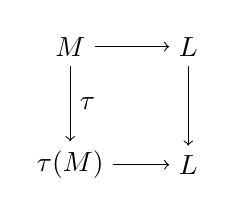
\begin{tikzpicture}[node distance=1.5cm, auto]
    \node (M)    {$M$};
    \node (L) [right of=M] {$L$};
    \node (t) [below of=M] {$\tau(M)$};
    \node (L2) [below of=L] {$L$};

    \draw[->] (M) to node {$ $} (L);
    \draw[->] (M) to node {$\tau$} (t);
    \draw[->] (t) to node {$ $} (L2);
    \draw[->] (L) to node {$ $} (L2);
  \end{tikzpicture}

  with $\sigma$ yet to be formed.

  By Theorem \ref{9.6}, $\exists$ isomorphism $\sigma: L \longrightarrow L$ such that $\sigma \biggr\vert_M = \tau$.\\
  Therefore, $\sigma$ is an automorphism of $L$, and since $\sigma\biggr\vert_K = \tau\biggr\vert_K=id$, $\sigma$ is a $K$-automorphism of $L$.
\end{proof}

\begin{prop}{11.4} \label{11.4}
  $L:K$ finite normal, $\alpha,~\beta$ are zeros in $L$ of the irreducible polynomial $p \in K[t]$.

  Then, $\exists$ a $K$-automorphism $\sigma$ of $L$ such that $\sigma(\alpha)=\beta$.
\end{prop}
\begin{proof}
  By Corollary \ref{5.13}, $\exists$ isomorphism $\tau: K(\alpha) \longrightarrow K(\beta)$ such that $\tau \biggr\vert_K$ is the identity, and $\tau(\alpha)=\beta$.

  By Theorem \ref{11.3}, $\tau$ extends to a $K$-automorphism $\sigma$ of $L$.
\end{proof}

\begin{lemma}{11.8} \label{11.8}
  $K \subseteq L \subseteq N \subseteq M$, $L:K$ finite, $N$ normal closure of $L:K$.\\
  Let $\tau$ any $K$-monomorphism $\tau: L \longrightarrow M$.\\
  Then $\tau(L) \subseteq N$.
\end{lemma}
\begin{proof}
  $\alpha \in L$, $m$ minimal polynomial of $\alpha$ over $K$.\\
  $\Longrightarrow ~~ m(\alpha)=0$, so $\tau(m(\alpha))=0$

  (since $\tau$ is a $K$-automorphism, ie. maps the zeros of $m(t)$).\\

  Since $\tau$ is a $K$-monomorphism, $\tau(m(\alpha))=m(\tau(\alpha))=0$

  $\Longrightarrow~~ \tau(\alpha)$ is a zero of $m$.\\

  Therefore, $\tau(\alpha)$ lies in $N$, since $N:K$ is normal.\\
  Henceforth, $\tau(L) \subseteq N$.
\end{proof}

\begin{thm}{11.9}
  The following are equivalent:
  \begin{enumerate}
    \item $L:K$ normal
    \item $\exists$ finite normal extension $N$ of $K$ containing $L$,\\
      such that every $K$-monomorphism $\tau: L \longrightarrow N$ is a $K$-automorphism of $L$.
    \item for every finite extension $M$ of $K$ containing $L$,\\
      every $K$-monomorphism $\tau: L \longrightarrow M$ is a $K$-automorphism of $L$.
  \end{enumerate}
\end{thm}

\begin{thm}{11.10}
  $[L:N]=1,~ N$ normal closure of $L:K$. Then,

  $\exists~ n~ K$-monomorphisms $L \longrightarrow N$.\\
  (the ones proven by Lemma \ref{11.8}).
\end{thm}

\begin{cor}{11.11} \label{11.11}
  $|\Gamma(L:K)| = [L:K]$ (if $L:K$ is normal).

  ie. there are precisely $[L:K]$ distinct $K$-automorphisms of $L$.
\end{cor}

\begin{thm}{11.12}
  $\Gamma(L:K) = G$. If $L:K$ normal, then $K$ is the fixed field of $G$.
\end{thm}
\begin{proof}
  let $K_0$ be the fixed field of $G$. Let $[L:K]=n$.\\
  By \ref{11.11}, $|G| = [L:K] = n$.\\
  By \ref{10.5}, $[L:K_0]=n$ ($K_0$ fixed field).\\
  Since $K \subseteq K_0$, we must have $K=K_0$.

  $\Longrightarrow$ thus $K$ is the fixed field of $G$.
\end{proof}

\begin{thm}{11.14}
  if $L$ any field, $G$ any finite group of automorphisms of $L$, and $K$ its fixed field,

  then $L:K$ is \emph{finite} and \emph{normal}, with Galois group $G$.
\end{thm}


\begin{thm}{12.2}(Fundamental Theorem of Galois Theory)
  if $L:K$ finite and normal inside $\mathbb{C}$, with $\Gamma(L:K)=G$, then:
  \begin{enumerate}
    \item $|\Gamma(L:K)| = [L:K]$
      (by Corollary \ref{11.11})
    \item the maps * and $\dagger$ are mutual inverses, and setup an order-reversing one-to-one correspondence between $\mathcal{F}$ and $\mathcal{G}$.
    \item if $M$ an intermediate field, then
      $$[L:M] = |M^*|~~~~~~~ [M:K]=\frac{|G|}{|M^*|}$$
    \item for $M$ an intermediate field, $M:K$ normal iff
      $$\underbrace{\Gamma(M:K)}_{=M^*} \lhd \underbrace{\Gamma(L:K)}_{=G}$$
    \item for $M$ intermediate, if $M:K$ normal, then
      $$\Gamma(M:K) \cong \frac{G}{M^*}$$
      ie.
      $$\Gamma(M:K) \cong \frac{\Gamma(L:K)}{\Gamma(L:M)}$$
  \end{enumerate}
\end{thm}
\begin{proof}
  TODO
\end{proof}

\subsection{Chapter 13 - Full example}

(Chapter 13 is basically a full example. More examples can be found at section \ref{ex:galoisgroups})


\subsection{Detour: Isomorphism Theorems}
\begin{thm}{i.1}(\emph{First Isomorphism Theorem}) \label{1stisothm}

  \begin{minipage}{0.75\textwidth}
  If $\psi: G \longrightarrow H$ a group homomorphism, then $ker(\psi) \triangleleft G$.\\
  Let $\phi: G \longrightarrow G/ker(\psi)$ be the canonical homomorphism.\\
  Then $\exists$ unique isomorphism $\eta: G/ker(\psi) \longrightarrow \psi(G)$ such that $\psi = \eta \phi$.\\
  $\Longleftrightarrow$ ie. $G/ker(\psi) \cong \psi(G)$.
  \end{minipage}
\hfill
\begin{minipage}{0.2\textwidth}
  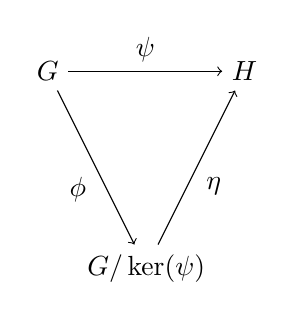
\begin{tikzpicture}[node distance=2.5cm, auto]
    \node (G)    {$G$};
    \node (H) [right of=G] {$H$};
    \node (GmodK) [below of=G, xshift=1.25cm] {$G/\ker(\psi)$};

    \draw[->] (G) to node {$\psi$} (H);
    \draw[->] (G) to node [swap] {$\phi$} (GmodK);
    \draw[->] (GmodK) to node [swap] {$\eta$} (H);
  \end{tikzpicture}
\end{minipage}
\end{thm}
\begin{proof}
  \emph{(proof from Thomas W. Judson book "Abstract Algebra" \cite{judson})}\\

  Let $K=ker(\psi)$.
  Since
  $$\eta: G/K \longrightarrow \psi(G)$$
  let
  $$\eta: gK \longrightarrow \psi(g)$$
  ie. $\eta(gK)=\psi(g)$.

  \begin{enumerate}[i.]
    \item show that $\eta$ is a \emph{well defined} map:

      if we have two representatives of the same coset, ie. $g_1 K=g_2 K$, we want to show that $\eta(g_1 K) = \eta(g_2 K)$, so that $\eta$ is a well-defined map.
      
      \vspace{0.3cm}
      By the coset properties for some $k \in K$, $g_1=g_2 k$, so

      $$\eta(g_1K)=\psi(g_1) = \psi(g_2 k) = \eta(g_2 k K) = \eta(g_2 K)$$

      Thus, $\eta$ does not depend on the choice of coset representatives, and
      the map $\eta: G/ker(\psi) \longrightarrow \psi(G)$ is uniquely defined
      since $\psi=\eta\phi$.

    \item show that $\eta$ is a homomorphism:

      Observe:
      $$\eta(g_1 K g_2 K) = \eta(g_1 g_2 K) = \psi(g_1 g_2) = \psi(g_1) \psi(g_2) = \eta(g_1 K) \eta(g_2 K)$$
      $\Longrightarrow$ so $\eta$ is a homomorphism.

    \item show that $\eta$ is an isomorphism:

      Since each element of $H=\psi(G)$ has at least a preimage, then $\eta$ is \emph{surjective} (onto $\psi(G)$).

      Show that it is also \emph{injective} (onet-to-one):
      
      Suppose 2 different preimatges lead to the same image in $\psi(G)$, ie.
      $\eta(g_1 K) = \eta(g_2 K)$

      then,
      $$\psi(g_1) = \psi(g_2)$$
      which implies $\psi(g_1^{-1} g_2) = e$, ie. $g_1^{-1} g_2 \in ker(\psi)$,
      hence
      $$g_1^{-1} g_2 K = K$$
      $$g_1 K = g_2 K$$
      so $\eta$ is injective.
  \end{enumerate}

  Since $\eta$ is injective and surjective $\Longrightarrow$ $\eta$ is a bijective homomorphism,\\
  ie. $\eta$ is an \emph{isomorphism}.
\end{proof}


\begin{thm}{i.2}(\emph{Second Isomorphism Theorem}) \label{2ndisothm}
  Let $H \subseteq G$, $N \triangleleft G$. Then
  \begin{enumerate}[i.]
    \item $HN \subseteq G$
    \item $H \cap N \triangleleft H$
    \item $\frac{H}{H \cap N} \cong \frac{HN}{N}$
  \end{enumerate}
\end{thm}
\begin{proof}
  \emph{(proof from Thomas W. Judson book "Abstract Algebra" \cite{judson})}\\

  \begin{enumerate}[i.]
    \item show $HN \subseteq G$:\\
      Note that $HN = \{ hn : h\in H, n\in N \}$. Let $h_1 n_1, h_2 n_2 \in HN$.

      Since $N$ normal $\Longrightarrow~ h_2^{-1} n_1 h_2 \in N$, so
      $$(h_1 n_1)(h_2 n_2) = h_1 h_2 (h_2^{-1} n_1 h_2) \cdot n_2 \in HN$$

      [Recall: since $N \triangleleft G$, $gN=Ng ~\forall g \in G$ $\Longrightarrow gn=n'g$ for some $n' \in N$.]

      To see that $(hn)^{-1} \in HN$:\\
      since $(hn)^{-1} = h^{-1} n^{-1} = h^{-1} (h n^{-1} h^{-1})$, thus $(hn)^{-1} \in HN$.

      Thus $HN \subseteq G$.


      In fact, $$HN = \bigcup_{h \in H} hN$$

      (TODO: diagram)

    \item show that $H \cap N \triangleleft H$:\\
      Let $h \in H,~ n \in H \cap N$ (recall: $H \cap N \subseteq H$).\\
      Then $h^{-1}nh \in H$ $\longleftarrow$ since $h^{-1}, n, h \in H$.\\
      Since $N \triangleleft G$, $h^{-1} n h \in N$.\\
      Therefore, $h^{-1}nh \in H \cap N$ $\Longrightarrow~ H \cap N \triangleleft H$

    \item show that $\frac{H}{H \cap N} \cong \frac{HN}{N}$:\\
      Define a map
      \begin{align*}
	\phi: &H \longrightarrow \frac{HN}{N}\\
	\text{by}~ \phi: &h \longmapsto hN
      \end{align*}

      $\phi$ is surjective (onto), since any coset $hnN=hN$ is the image of $h \in H$, ie. $\phi(h)$

      $\phi$ is a homomorphism, since
      $$\phi(h h') = h h' N = hN h'N = \phi(h)\phi(h')$$

      By the First Isomorphism Theorem \ref{1stisothm},
      $$\frac{HN}{N} \cong \frac{H}{ker(\phi)}$$

      and since
      \begin{align*}
	&ker(\phi) = \{ h \in H : h \in N\}\\
	&\text{then}~~ker(\phi) = H \cap N
      \end{align*}

      so then,
      $$\frac{HN}{N} = \phi(H) \cong \frac{H}{ker(\phi)} = \frac{H}{H \cap N}$$
      thus
      $$\frac{HN}{N} \cong \frac{H}{H \cap N}$$

  \end{enumerate}
\end{proof}


\begin{thm}{i.3}(\emph{Third Isomorphism Theorem}) \label{2ndisothm}\\
  Let $H \subseteq K$ and $K \triangleleft G,~ H \triangleleft G$.\\
  Then
  $\frac{K}{H} \triangleleft \frac{G}{H}$
  and
  $$\frac{ G/H }{ K/H } \cong \frac{G}{K}$$
\end{thm}
\begin{proof}
  \emph{(proof from Dummit and Foote book ``Abstract Algebra" \cite{dummitfoote})}\\

  Easy to see that $\frac{K}{H} \triangleleft \frac{G}{H}$.

  Define
      \begin{align*}
	\psi: &\frac{G}{H} \longrightarrow \frac{G}{K}\\
	\text{by}~ \psi: &gH \longmapsto gK
      \end{align*}

  To show that $\psi$ is \emph{well defined}:\\
  suppose $g_1 H = g_2 H$, then $g_1 = g_2 h$ for some $h \in H$.\\
  Since $H \subseteq K \Longrightarrow~ h \in K$, hence $g_1 K = g_2 K$,\\
  ie. $\psi(g_1 H) = \psi(g_2 H)$, which shows that $\psi$ is well defined.

  Since $g \in G$ may be chosen arbitrarily in $G$, $\psi$ is a surjective homomorphism.


  Finally,
  \begin{align*}
    ker(\psi) &= \{ gH \in \frac{G}{H} \mid \psi(gH)=1K \}\\
    &= \{ gH \in \frac{G}{H} \mid gK =1K \}\\
    &= \{ gH \in \frac{G}{H} \mid g \in K \}\\
    &= \frac{K}{H}
  \end{align*}


  By the First Isomorphism Theorem (\ref{1stisothm}),

  \begin{tikzpicture}[node distance=2.5cm, auto]
    \node (GmodH)    {$\frac{G}{H}$};
    \node (GmodK) [right of=GmodH] {$\frac{G}{K}$};
    \node (GmodHmodKer) [below of=G, xshift=1.25cm] {$\frac{G/H}{\ker(\psi)} = \frac{G/H}{K/H}$};

    \draw[->] (GmodH) to node {$\psi$} (GmodK);
    \draw[->] (GmodH) to node [swap] {$\phi$} (GmodHmodKer);
    \draw[->] (GmodHmodKer) to node [swap] {$\eta$} (GmodK);
  \end{tikzpicture}

  So, by
  $$\eta: \frac{G/H}{K/H} \longrightarrow \frac{G}{K}$$
  since $\eta$ is
  bijective (we know it by the First Isomorphism Theorem), $\eta$ it is the isomorphism:
  $$\frac{ G/H }{ K/H } \cong \frac{G}{K}$$


\end{proof}

\subsection{Chapter 14}

\begin{defn}{14.1} \label{14.1}
  a group $G$ is soluble if it has a finite series of subgroups
  $$1=G_0 \subseteq G_1 \subseteq \ldots \subseteq G_n = G$$
  such that
  \begin{enumerate}[i.]
    \item $G_i \lhd G_{i+1}$ for $i=0,\ldots,n-1$
    \item $\frac{G_{i+1}}{G_{i+1}}$ is Abelian for for $i=0,\ldots,n-1$
  \end{enumerate}

  (Note: $G_i \lhd G_{i+1} \lhd G_{i+2}$ does not imply $G_i \lhd G_{i+2}$)
\end{defn}

\begin{thm}{14.4}
  $H \subseteq G,~~ N \triangleleft G$, then
  \begin{enumerate}
    \item if $G$ soluble $\Longrightarrow H$ soluble
    \item if $G$ soluble $\Longrightarrow G/N$ soluble
    \item if $N$ and $G/N$ soluble $\Longrightarrow G$ soluble
  \end{enumerate}
\end{thm}
\begin{proof}
  \begin{enumerate}
    \item Since $G$ soluble, by definition: $\exists~~ 1=G_0 \triangleleft G_1 \triangleleft \ldots \triangleleft G_r = G$ with Abelian quotients $\frac{G_{i+1}}{G_i}$.

      Let $H_i = G_i \cap H$, then $H$ has a series $1=H_0 \triangleleft H_1
      \triangleleft \ldots \triangleleft H_r = H$, next we show that the
      quotients $\frac{H_{i+1}}{H_i}$ are Abelian (so that H is soluble):

      $$\frac{H_{i+1}}{H_i} = \frac{G_{i+1} \cap H}{G_i \cap H} \stackrel{(*)}{=} \frac{G_{i+1} \cap H}{G_i \cap (G_{i+1}\cap H)}
      \stackrel{(**)}{\cong} \frac{G_i(G_{i+1} \cap H)}{G_i} \subseteq \frac{G_{i+1}}{G_i}
      $$

      (*): to see why, $H_i = G_i \cap H = G_i \cap H_i = G_i \cap H_{i+1} = G_i \cap (G_{i+1} \cap H)$.
      (**): by the 2nd Isomorphism Theorem (\ref{2ndisothm}).

      [TODO: diagram of subgroups] % TODO %
      
      Notice that $\frac{G_{i+1}}{G_i}$ is Abelian, thus the left-hand-side of the congruence is also Abelian.
      Therefore, $\frac{H_{i+1}}{H_i}$ is Abelian, thus $H$ is soluble.

    \item For $G/N$ to be soluble, (by definition) it would have the series $\frac{N}{N} = G_0 \frac{N}{N} \triangleleft G_1 \frac{N}{N} \triangleleft \ldots \triangleleft G_r \frac{N}{N} = \frac{G}{N}$,
      and any quotient being $\frac{G_{i+1}\frac{N}{N}}{G_i \frac{N}{N}}$.

      The series clearly exists, so now we show that the quotients are Abelian, so that $G/N$ is soluble:

      $$
      \frac{G_{i+1} N}{G_i N} = \frac{G_{i+1}(G_i N)}{G_i N} \stackrel{(*)}{\cong}
      \frac{G_{i+1}}{G_{i+1} \cap (G_i N)} \cong \frac{G_{i+1}/G_i}{(G_{i+1}
      \cap (G_i N))/G_i}
      $$

      (*): by the 2nd Isomorphism Theorem (\ref{2ndisothm}).

      The last quotient is a quotient of the Abelian group $G_{i+1}/G_i$, so it is Abelian.

      Hence, $\frac{G_{i+1}N}{G_i N}$ is also Abelian; so $\frac{G}{N}$ is soluble.

    \item
      By the definition of $N$ and $G/N$ being soluble,
      \begin{align*}
	N \text{soluble} \Longrightarrow~~ 1 &= N_0 \triangleleft N_1 \triangleleft \ldots \triangleleft N_r = N\\
	G/N \text{soluble} \Longrightarrow~~ 1= \frac{N}{N} &= \frac{G_0}{N} \triangleleft \frac{G_1}{N} \triangleleft \ldots \triangleleft \frac{G_r}{N} = \frac{G}{N}
    \end{align*}
    both with Abelian quotients.

    Consider the series of $G$ given by combining the two previous series:

    $$
      1 = N_0 \triangleleft N_1 \triangleleft \ldots \triangleleft N_r = N = G_0 \triangleleft G_1 \triangleleft \ldots \triangleleft G_r = G
    $$
    the quotients are either
    \begin{itemize}
      \item $\frac{N_{i+1}}{N_i}$, Abelian
      \item $\frac{G_{i+1}}{G_i}$, isomorphic to $\frac{G_{i+1}/N}{G_i/N}$,
	which is Abelian.
    \end{itemize}
  \end{enumerate}
  Therefore, the quotients are always Abelian; hence $G$ is soluble.
\end{proof}


\begin{defn}{14.5}
  $G$ is \emph{simple} if it's nontrivial and it's only normal subgroups are $1$ and $G$.
\end{defn}

\begin{thm}{14.6} \label{14.6}
  A \emph{soluble} group is \emph{simple} iff it is cyclic of prime order.
\end{thm}
\begin{thm}{14.7} \label{14.7}
  if $n \geq 5$, then $\mathbb{A}_n$ is simple.
\end{thm}
\begin{cor}{14.8}
  $\mathbb{S}_n$ is not soluble if $n \geq 5$.
\end{cor}
\begin{proof}
  if $\mathbb{S}_n$ were soluble, then $\mathbb{A}_n$ would be soluble by Theorem \ref{14.1}(i), and simple by Theorem \ref{14.7}, hence of prime order by Theorem \ref{14.6}.
  
  But observe: $|\mathbb{A}_n|=\frac{1}{2}(n!)$ is not prime if $n \geq 5$.\\
  Thus $\mathbb{S}_n$ is not soluble if $n \geq 5$.
\end{proof}

\begin{lemma}{14.14} \label{14.14}
  if $A$ finite and abelian group with $p \biggr\vert |A|$ ($p$ prime), then $A$ has an element of order $p$.
\end{lemma}
\begin{proof}
  \begin{enumerate}[i.]
    \item if $|A|$ prime and Abelian $\Longrightarrow$ then $A$ is cyclic.

      Since $p \vert |A| ~~ \Longrightarrow ~~ \exists! ~ B \subseteq A$ such that $|B|=p$, where $B = <b>$ with $ord(b)=p$. So the lemma is proven.

    \item if $|A|$ non-prime:

      take $M \subseteq A$ with $|M|=m$, $m$ maximal. Then

      \begin{enumerate}[a.]
	\item if $p|m ~~ \Longrightarrow ~~ \exists! ~ B'=<b'>,~ b' \in A$ with $|B'|=p$ and $ord(b')=p$.
	\item if $p \nmid m$:
	  Let $b \in A \not M$ and $B=<b>$.\\
	  Then $MB \supseteq M$, and by maximility must be $MB=A$.

	  By the 1st Isomorphism Theorem (\ref{1stisothm}),
	  $$|A| = |MB| = \frac{|M| \cdot |B|}{|M \cap B|}$$
	  both $|A|$ and $|B|$ are divisible by $p$ (but recall that $p \nmid m=|M|$), since $B$ is cyclic and $p \vert |B|$

	  $\Longrightarrow$ thus, $B$ has an element of order $p$.
	  
	  So, if $|B|=r$, and $p|r ~~ \Longrightarrow~~ ord(b^{r/p}) = p$.\\

	  Hence, in all cases i, ii.a, ii.b, $A$ contains an element of order $p$.
      \end{enumerate}
  \end{enumerate}
\end{proof}

\begin{thm}{14.15}(Cauchy's Theorem)
  if $p \biggr\vert |G|$ ($p$ prime), then $\exists ~ x \in G$ such that $ord(x)=p$.
\end{thm}
\begin{proof}
  (induction on $|G|$)

  For $|G|=1,2,3$, trivial.

  Induction step: class equation
  $$|G|=1+|C_2|+ \ldots + |C_r|$$
  since $p \biggr\vert |G|$, must have $p \nmid |C_j|$ for some $j \geq 2$.

  If $x \in C_j ~~\Longrightarrow p \biggr\vert |C_G(x)|$ (since $|C_j|=|G|/|C_G(x)|$, recall $p\biggr\vert |G|$).

  \begin{enumerate}[i.]
    \item if $C_G(x) \neq G$:\\
      (by induction) since $p \biggr\vert |C_G(x)|$,

      $\exists a \in C_G(x)$ with $ord(a)=p$, and $a \in G$ (since $C_G(x) \subset G$).
    \item otherwise, $C_G(x)=G$:\\
      implies $x \in Z(G)$, by choice $x\neq 1$, so $Z(G)\neq 1$.

      Then either
      \begin{enumerate}[I.]
	\item $p \biggr\vert |Z(G)| ~~ \longrightarrow$ Abelian case, Lemma \ref{14.14}.
	\item $p \not\biggr\vert |Z(G)|$:
	  by induction, $\exists x \in G$ such that $\hat{x} \in G/Z(G)$, with $ord(\hat{x})=p$. (where $\hat{x}$ is the image of $x$).

	  $\Longrightarrow~~ x^p \in Z(G)$, but $x \not\in Z(G)$.

	  Let $X=<x>$, cyclic.\\
	  $XZ(G)$ is Abelian, and $p \biggr\vert |XZ(G))|$\\
	  $\Longrightarrow$ by Lemma \ref{14.14}, it has an element of order $p$, and this element belongs to $G$.
      \end{enumerate}

  \end{enumerate}
\end{proof}

\begin{defn}{15.1}(Soluble by radicals)
  let $f \in K[t],~ K \subseteq \mathbb{C}$, and $\Sigma$ a splitting field of $f$ over $K$.

  $f$ is \emph{soluble by radicals} if\\
  $\exists$ a field $M$ with $\Sigma \subseteq M$ such that $M:K$ is a radical extension (\ref{8.12}).

  Note: not required $\Sigma:K$ to be radical.
\end{defn}

\begin{lemma}{15.3}
  $L:K$ radical extension $\mathbb{C}$, and $M$ normal enclosure of $L:K$, then $M:K$ is radical.
\end{lemma}
\begin{proof}
  let $L=K(\alpha_1, \ldots, \alpha_r)$ with $\alpha_i^{n_i} \in K(\alpha_1, \ldots, \alpha_{j-1})$ (by definition of $L:K$ being a radical extension).

  Let $f_i$ be the minimal polynimal of $\alpha_i$ over $K$.

  Then, $M \supseteq L$ is splitting field of $\Prod_{i=1}^r f_i$, since $M$ is normal enclosure of $L:K$.

  For every zero $\beta_{ij}$ of $f_i$ in $M$,\\
  $\exists$ an isomorphism $\sigma: K(\alpha_i) \longrightarrow K(\beta_{ij})$ by Corollary \ref{5.13}.

  By Proposition \ref{11.4}, since $K(\alpha_i),~K(\beta_{ij}) \subset M$,
  $\sigma$ extends to a $K$-automorphism
  $$\tau: M \longrightarrow M$$
  since $M$ is splitting field (ie. contains the zeros of $\Prod f_i$).

  Since $\alpha$ is a member of radical sequence for a subfield of $M$, so it is $\beta_{ij}$.

  By combining the sequences for $M$, $M:K$ is a radical extension.
\end{proof}


\vspace{0.5cm}

The next two lemmas show that certain Galois groups are Abelian.

\begin{lemma}{15.4}
\end{lemma}
\begin{proof}
\end{proof}

\newpage

\section{Tools}
This section contains tools that I found useful to solve Galois Theory related problems, and that don't appear in Stewart's book.

\subsection{De Moivre's Theorem and Euler's formula}\label{demoivre}
Useful for finding all the roots of a polynomial.

Euler's formula:
$$e^{i \psi} = cos \psi + i \cdot sin \psi$$

The n-th roots of a complex number $z=x + i y = r (cos \theta + i \cdot sin \theta)$ are given by

$$z_k = \sqrt[n]{r} \cdot \left(cos(\frac{\theta + 2k \pi}{n}) + i \cdot sin(\frac{\theta + 2k \pi}{n}) \right)$$
for $k=0, \ldots, n-1$.

So, by Euler's formula:
$$z_k = \sqrt[n]{r} \cdot e^{i (\frac{\theta + 2 k \pi}{n})}$$

Usually we will set $\alpha=\sqrt[n]{r}$ and $\zeta = e^{\frac{2 \pi i}{n}}$,
and find the $\mathbb{Q}$-automorphisms from there (see \ref{ex:galoisgroups} for examples).

\subsection{Einsenstein's Criterion} \label{einsenstein}
\emph{reference: Stewart's book}

Let $f(t) = a_0 + a_1 t + \ldots + a_n t^n$, suppose there is a prime $q$ such that
\begin{enumerate}
  \item $q \nmid a_n$
  \item $q | a_i$ for $i=0, \ldots, n-1$
  \item $q^2 \nmid a_0$
\end{enumerate}
Then, $f$ is irreducible over $\mathbb{Q}$.

\emph{TODO proof \& Gauss lemma.}


\subsection{Elementary symmetric polynomials}
\emph{TODO from orange notebook, page 36}

\subsection{Cyclotomic polynomials} \label{cyclotomicpoly}
\subsubsection{From Elmyn Berlekamp's "Algebraic Coding Theory" book}
The notes in this section are from the book "Algebraic Coding Theory" by Elmyn
Berlekamp \cite{berlekamp}.

\vspace{0.3cm}

Some times we might find polynomials that have the shape of $t^n - 1$, those are \emph{cyclotomic polynomials}, and have some properties that might be useful.

Observe that in a finite field of order $q$, factoring $x^q - x$ gives
$$x^q-x = x(x^{q-1} -1)$$

The factor $x^{q-1} -1$ is a special case of $x^n -1$: if we assume that the
field contains an element $\alpha$ of order $n$, then the roots of $x^n-1=0$ are
$$1, \alpha, \alpha^2, \alpha^3, \ldots, \alpha^{n-1}$$
and $\deg(x^n-1)=n$, thus $x^n-1$ has at most $n$ roots in any field, henceforth
the powers of $\alpha$ must include all the $n$-th roots of unity.

There fore, in any field which contains a primitive $n$-th root of unity we have:

\begin{thm}{4.31}
  $$x^n -1 = \prod_{i=0}^{n-1} (x - \alpha^i) = \prod_{i=1}^n (x-\alpha^i)$$
\end{thm}

If $n=k \cdot d$, then $\alpha^k, \alpha^{2k}, \alpha^{3k}, \ldots, \alpha^{dk}$ are all roots of $x^d -1 =0$

Every element with order dividing $n$, must be a power of $\alpha$, since an
element of order $d$ is a $d$-th root of unity.

Every power of $\alpha$ has order which divides $n$, and every field element
whose order divides $n$ is a power of $\alpha$. This suggests that we partition
the powers of $\alpha$ according to their orders:
$$x^n -1 = \prod_{\stackrel{d,}{d|n}} \prod_{\beta} (x- \beta)$$
where at each iteration, $\beta$ is a field element of order $d$ for each $d$.

The polynomial whose roots are the field elements of order $d$ is called the
\emph{cyclotomic polynomial}, denoted by $Q^{(d)}(x)$.

\begin{thm}{4.32}
  $$x^n -1 = \prod_{\stackrel{d,}{d|n}} Q^{(d)}(x)$$
\end{thm}


\subsubsection{From Ian Stewart's ``Galois Theory'' book}
Notes from Ian Stewart's book \cite{ianstewart}.

Consider the case $n=12$, let $\zeta=e^{\pi i /6}$ be a primitive $12$-th root of unity.
Classify its powers ($\zeta^j$) according to their minimal power $d$ such that
$(\zeta^j)^d = 1$ (ie. when they are primitive $d$-th roots of unity).

\begin{enumerate}[]
  \item $d=1,~~~ 1$
  \item $d=2,~~~ \zeta^6$
  \item $d=3,~~~ \zeta^4, \zeta^8$
  \item $d=4,~~~ \zeta^3, \zeta^9$
  \item $d=6,~~~ \zeta^2, \zeta^{10}$
  \item $d=12,~~~ \zeta, \zeta^5, \zeta^7, \zeta^{11}$
\end{enumerate}

Observe that we can factorize $t^{12} -1$ by grouping the corresponding zeros:
\begin{align*}
  t^{12}-1 = &(t-1) \times\\
	     &(t-\zeta^6) \times\\
	     &(t-\zeta^4) (t-\zeta^8) \times\\
	     &(t-\zeta^3) (t-\zeta^9) \times\\
	     &(t-\zeta^2) (t-\zeta^{10}) \times\\
	     &(t-\zeta) (t-\zeta^5)(t-\zeta^7) (t-\zeta^{11})
\end{align*}
which simplifies to
$$t^{12}-1=(t-1)(t+1)(t^2+t+1)(t^2+1)(t^2-t+1)F(t)$$
where $F(t) = (t-\zeta) (t-\zeta^5)(t-\zeta^7) (t-\zeta^{11}) = t^4 -t^2 + 1$ (this last step can be obtained either by multiplying $(t-\zeta)(t-\zeta^5)(t-\zeta^7) (t-\zeta^{11})$ together, or by dividing $t^{12}-1$ by all the other factors).


Let $\Phi_d(t)$ be the factor corresponding to primitive $d$-th roots of unity, then we have proved that
$$t^{12}-1 = \Phi_1 \Phi_2 \Phi_3 \Phi_4 \Phi_6 \Phi_{12}$$


\begin{defn}{21.5}
  The polynomial $\Phi_d(t)$ defined by
  $$\Phi_n(t) = \prod_{a\in \mathbb{Z}_n,(a,n)=1} (t- \zeta^a)$$
  is the $n$-th \emph{cyclotomic polynomial} over $\mathbb{C}$.
\end{defn}

\begin{cor}{21.6}
  $\forall n \in \mathbb{N}$, the polynomial $\Phi_n(t)$ lies in $\mathbb{Z}[t]$ and is monic and irreducible.
\end{cor}

\begin{thm}{21.9}
  \begin{enumerate}
    \item The Galois group $\Gamma(\mathbb{Q}(\zeta):\mathbb{Q})$ consists of the
    $\mathbb{Q}$-automorphisms $\psi_j$ defined by
    $$\psi_j(\zeta)=\zeta^j$$
    where $0 \leq j \leq n-1$ and $j$ is prime to $n$.

    \item $\Gamma(\mathbb{Q}(\zeta):\mathbb{Q}) \stackrel{iso}{\cong} \mathbb{Z}_n^*$, and is an abelian group.
    \item its order is $\phi(n)$
    \item if $n$ is prime, $\mathbb{Z}_n^*$ is cyclic
  \end{enumerate}
\end{thm}



\vspace{1cm}

\subsubsection{Examples}
Examples of cyclotomic polynomials:

\begin{align*}
  \Phi_n(x) &= x^{n-1} + x^{n-2} + \ldots + x^2 + x + 1 = \sum_{i=0}^{n-1} x^i\\
  \Phi_{2p}(x) &= x^{p-1} + \ldots + x^2 - x + 1 = \sum_{i=0}^{p-1} (-x)^i\\
  \Phi_m(x) &= x^{m/2} + 1, ~~\text{when $m$ is a power of $2$}
\end{align*}


\subsection{Lemma 1.42 from J.S.Milne's book}
Lemma from J.S.Milne's book \cite{milneFT}.

Useful for when dealing with $x^p - 1$ with $p$ prime.

Observe that

$$x^p -1 = (x-1)(x^{p-1} + x^{p-2} + \ldots + 1)$$

Notice that
$$\Phi_p(x) = x^{p-1} + x^{p-2} + \ldots + 1$$
is the $p$-th Cyclotomic polynomial.

\begin{lemma}{1.42}
  If $p$ prime, then $x^{p-1} + \ldots + 1$ is irreducible; hence $\mathbb{Q}[e^{2 \pi i /p}]$ has degree $p-1$ over $\mathbb{Q}$.
\end{lemma}
\begin{proof}
  Let $f(x) = (x^p - 1)/(x-1) = x^{p-1} + \ldots + 1$
  then
  $$
  f(x+1) = \frac{(x+1)^p -1}{x+1-1} = \frac{(x+1)^p -1}{x} = x^{p-1} + \ldots + a_i x^i + \ldots + p
  $$

  with $a_i = \left( \stackrel{p}{i+1} \right)$.

  We know that $p | a_i$ for $i= 1, \ldots, p-2$, therefore $f(x+1)$ is irreducibe by Einsenstein's Criterion.

  This implies that $f(x)$ is irreducible.
\end{proof}


\subsection{Dihedral groups - Groups of symmetries} \label{dihedral}
Source: Wikipedia and \cite{dihedral}.

Dihedral groups ($\mathbb{D}_n$) represent the symmetries of a regular $n$-gon.

Properties:
\begin{itemize}
  \item are non-abelian (for $n>2$), ie. $rs \neq sr$
  \item order $2n$
  \item generated by a rotation $r$ and a reflection $s$
  \item $r^n = s^2 = id,~~~(rs)^2=id$
\end{itemize}
Subgroups of $\mathbb{D}_n$:
\begin{itemize}
  \item rotation form a cyclic subgroup of order $n$, denoted as $<r>$
  \item for each $d$ such that $d|n$, $\exists~ \mathbb{D}_d$ with order $2d$
  \item normal subgroups
    \begin{itemize}
      \item for $n$ odd: $\mathbb{D}_n$ and $<r^d>$ for every $d|n$
      \item for $n$ even: $2$ additional normal subgroups
    \end{itemize}
  \item Klein four-groups: $\mathbb{Z}_2 \times \mathbb{Z}_2$, of order 4
\end{itemize}

\vspace{0.3cm}
Total number of subgroups in $\mathbb{D}_n$: $d(n) + s(n)$, where $d(n)$ is the number of positive disivors of $n$, and $s(n)$ is the sum of those divisors.

\begin{eg}{}
For $\mathbb{D}_6$, we have $\{1,2,3,6\} | 6$, so $d(n) = d(6) = 4$, and
$s(6) = 1+2+3+6 = 12$; henceforth, the total amount of subgroups is $d(n)+s(n) = 4+12 = 16$.
\end{eg}

\vspace{0.3cm}
For $n \geq 3, ~~\mathbb{D}_n \subseteq \mathbb{S}_n$ (subgroup of the Symmetry group).

\subsection{Rolle's theorem} \label{rolle}

\begin{thm}{}(Rolle's Theorem)
  if a real-valued function $f$ is
  \begin{itemize}
    \item \emph{continuous} on a proper closed interval $[a,b]$
    \item \emph{differentiable} on the open interval $(a,b)$
    \item $f(a)=f(b)$
  \end{itemize}
  then, $\exists$ at least one $c$ in $(a,b)$ such that $Df(c)=0$.
\end{thm}
\begin{proof} (proof source: cue math website)
  Notice that when $Df(x_i)=0$ occurs, is a maximum or minimum (extrema) value of $f$.
  $\Longrightarrow$ if a function is continuous, it is guaranteed to have both a maximum and a minimum point in the interval.\\

  Two possibilities:
  \begin{enumerate}[i.]
    \item $f$ is constant\\
    $\Longrightarrow$ ie. a horizontal line ($f(a)=f(b)$), ie. no slope $\Longrightarrow$ $Df=0$ everywhere in $[a,b]$.
  \item $f$ is not constant:\\
    since $f$ not constant, must change directions in ordder to start and end at the same $y$-value ($f(a)=f(b)$).\\
    Thus at some point between $a$ and $b$ it will either have a minimum, maximum or both.
    \begin{enumerate}[a.]
      \item does the maximum occur at a point where $Df > 0$?\\
	No, because if $Df > 0$, then $f$ is increasing, but it can not increase since we're at its maximum point.
      \item does the maximum occur at a point where $Df < 0$?\\
	No, because if $Df < 0$, then $f$ is deccreasing, which means that at our left it was larger, but we're at a maximum point, so a contradiction.
    \end{enumerate}
    Same with minimus.\\
    $\Longrightarrow$ Hence, since $Df \nless 0$ and $Df \ngtr 0$, and $Df$ exists, then $Df=0$.
  \end{enumerate}
  \\
    Thus, $f$ must have extrema (either max or min or both), and at that extrema $Df$ must be zero.
\end{proof}


Consequence of Rolle's Theorem:

\begin{cor}{}(Zero separation property)
  Between any two distinct consecutive zeros of $f$, there lies at least one zero of $Df$.
\end{cor}
\begin{eg}{}
  If $f(t)$ has zeros $t_1, t_2$, with $t_1 < t_2$, and $f$ is derivable, then by Rolle'z theorem:

  $\exists c \in (t_1, t_2)$ such that $Df(c)=0$.

  Hence, the zeros of $Df$ \emph{separate} the zeros of $f$.
\end{eg}

\newpage

\section{Exercises}

\subsection{Galois groups}\label{ex:galoisgroups}

\subsubsection[t6-7]{$t^6-7 \in \mathbb{Q}$}

This exercise comes from a combination of exercises 12.4 and 13.7 from \cite{ianstewart}.

First let's find the roots. By De Moivre's Theorem (\ref{demoivre}), $t_k =
\sqrt[6]{7} \cdot e^{i \frac{2 \pi k}{6}}$.

From which we denote $\alpha = \sqrt[6]{7}$, and $\zeta = e^{\frac{2 \pi i}{6}}$, so that the
roots of the polynomial are $\{ \alpha, \alpha \zeta, \alpha \zeta^2, \alpha \zeta^3, \alpha \zeta^4, \alpha \zeta^5\}$, ie. 
$\{ \alpha \zeta^k \}_0^5$.

Hence the \emph{splitting field} is $\mathbb{Q}(\alpha, \zeta)$.

\emph{Degree of the extension}

In order to find $[\mathbb{Q}(\alpha, \zeta) : \mathbb{Q}$, we're going to split it in tow
parts. By the Tower Law (\ref{towerlaw}),

$$[\mathbb{Q}(\alpha, \zeta) : \mathbb{Q}] = [\mathbb{Q}(\alpha, \zeta) : \mathbb{Q}(\alpha)] \cdot [\mathbb{Q}(\alpha) : \mathbb{Q}]$$

To find each degree, we will find the minimal polynomial of the adjoined term over the base field of the extension:

\begin{enumerate}[i.]
  \item minimal polynomial of $\alpha$ over $\mathbb{Q}$\\
    By Einsenstein's Criterion (\ref{einsenstein}), with $q=7$ we have that $q
    \nmid 1$, $7 | {-7,0,0,\ldots}$, and $7^2 \nmid -7$, hence $f(t)$ is
    irreducibe over $\mathbb{Q}$, thus is the minimal polynomial
    $$m_i(t)= f(t) =t^6-7$$
    which has roots $\{ \alpha \zeta^k \}_0^5$.
  \item minimal polynomial of $\zeta$ over $\mathbb{Q}(\alpha)$\\
    Since $\zeta$ is the primitive $6$th root of unity, we know that the minimal
    polynomial will be the $6$th cyclotomic polynomial (\ref{cyclotomicpoly}):
    $$m_{ii}(t) = \Phi_6(t) = t^2 - t + 1$$
    which has roots $\zeta, -\zeta$.

    Since $\mathbb{Q}(\alpha) \subseteq \mathbb{R}$, and the roots of
    $\Phi_6(t)=t^2 - t +1$ are in $\mathbb{C}$, $\Phi_6(t)$ remains irreducible
    over $\mathbb{Q}(\alpha)$.
\end{enumerate}

\vspace{0.5cm}
Therefore, by the tower of law,
$$[\mathbb{Q}(\alpha, \zeta) : \mathbb{Q}] = \deg{\Phi_6(t)} \cdot \deg{f(t)} = 2 \cdot 6 = 12$$
and by the Fundamental Theorem of Galois Theory, we know that
$$|\Gamma( \mathbb{Q}(\alpha, \zeta) : \mathbb{Q} )| = [\mathbb{Q}(\alpha, \zeta) : \mathbb{Q}] = 12$$
which tells us that there exist $12$ $\mathbb{Q}$-automorphisms of the Galois group.


\vspace{0.5cm}
Let's find the $12$ $\mathbb{Q}$-automorphisms. Start by defining $\sigma$ which
fixes $\zeta$ and acts on $\alpha$, sending it to another of the roots of the
minimal polynomial of $\alpha$ over $\mathbb{Q}$, $f(t)$, choose $\alpha \zeta$.

Now define $\tau$ which fixes $\alpha$ and acts on $\zeta$, sending it into
another root of the minimal polynomial of $\zeta$ over $\mathbb{Q}(\alpha)$,
choose $-\zeta$.

\vspace{0.3cm}
\begin{tabular}{@{}l l@{}}
    $\begin{aligned}
      \sigma: \alpha &\mapsto \alpha \zeta \\
      \zeta &\mapsto \zeta
    \end{aligned}$
  &
    $\begin{aligned}
      \tau: \alpha &\mapsto \alpha\\
      \zeta &\mapsto -\zeta = \zeta^{-1}
    \end{aligned}$
\end{tabular}

In other words, we have $12$ $\mathbb{Q}$-automorphisms, which are the
combination of $\sigma$ and $\tau$:

$$\begin{aligned}
  \sigma^k \tau^j:~~&\alpha \mapsto \alpha \zeta^k\\
		    &\zeta \mapsto \zeta^j
\end{aligned}$$

for $0 \leq k \leq 5$ and $j = \pm 1$.

\vspace{0.5cm}

NOTE: WIP diagram.
\begin{tikzpicture}[node distance=2cm]
  \def \radius{2}
  \draw (0,0) circle (\radius);

  \foreach \k in {0,...,5} {
    % \node (a\k) at ({360/6 * \k}:\radius) {$\alpha \zeta^{\k}$};
    \node (a\k) at ({360/6 * \k}:\radius+0.5) {$\alpha \zeta^{\k}$};
    \fill ({360/6 * \k}:\radius) circle (2pt);
  }
  % real & im axis
  \draw[->] (-2.5,0) -- (2.5,0) node[right] {};
  \draw[->] (0,-2.5) -- (0,2.5) node[above] {};


  % tau:
  \draw[<->] (3,1) -- (3,-1) node[right] {$\tau$};
  % sigma:
  % \foreach \k [evaluate=\k as \next using int(mod(\k+1,6))] in {0,...,5} {
  %   \coordinate (p\k) at ({360/6 * \k}:\radius);
  %   \coordinate (p\next) at ({360/6 * \next}:\radius);
  % 
  %   \draw[->, bend left=30] (p\k.center) -- node[above] {$\sigma$} (p\next.center);
  % }
  \foreach \k in {0,...,5} {
    \coordinate (p\k) at ({360/6 * \k}:\radius);
  }
  \foreach \k [evaluate=\k as \next using int(mod(\k+1,6))] in {0,...,5} {
    \draw[->, bend left=30] (p\k) -- node[above] {$\sigma$} (p\next);
  }
\end{tikzpicture}

\vspace{0.5cm}

Observe, that $\Gamma$ is generated by the combination of $\sigma$ and $\tau$,
and it is isomorphic to the group of symmetries of order 12, the dihedral
group (\ref{dihedral}) of order 12, $\mathbb{D}_6$, ie. $\Gamma \cong \mathbb{D}_6$.

\vspace{0.5cm}

Let's find the subgroups of $\Gamma$, and the fixed fields of $\mathbb{Q}(\alpha, \zeta)$.

We know that $\Gamma \cong \mathbb{D}_6$, and we know from the properties
of the dihedral group (\ref{dihedral}) that the number of subgroups of
$\mathbb{D}_6$ will be $d(6) + s(6) = 4 + 12 = 16$ subgroups.


\vspace{0.4cm}

\hspace*{-3.5cm}
\begin{tabular}{ c c c c | p{7.5cm} }
  \hline
  generators & order & group & fixed field & notes (check fixed field)\\
\hline
  $\langle \rangle = \langle \sigma^6 \rangle=\langle \tau^2 \rangle$ & 1 & id & $\mathbb{Q}(\alpha,\zeta)$ & \\
  $\langle \sigma \rangle = \langle \sigma^5 \rangle$ & 6 & $\mathbb{Z}_6$ & $\mathbb{Q}(\zeta)$ & \\
  $\langle \sigma^2 \rangle=\langle \sigma^4 \rangle$ & 3 & $\mathbb{Z}_3$ & $\mathbb{Q}(\alpha^3, \zeta)$ & $\sigma^2(\alpha^3)=\alpha^3 \zeta^{3\cdot 2}=\alpha^3 \zeta^6 = \alpha^3 \cdot 1 = \alpha^3$\\
  $\langle \sigma^3 \rangle$ & 2 & $\mathbb{Z}_2$ & $\mathbb{Q}(\alpha^2,\zeta)$ & $\sigma^3(\alpha^2)=(\alpha\zeta^3)^2=\alpha^2\zeta^6=\alpha^2$\\
  \hline
  $\langle \tau \rangle$ & 2 & $\mathbb{Z}_2$ & $\mathbb{Q}(\alpha)$ & \\
  \hline
  $\langle \sigma\tau \rangle$ & 2 & $\mathbb{Z}_2$ & $\mathbb{Q}(\alpha+\alpha\zeta)$ &
      $\sigma\zeta(\alpha+\alpha\zeta)=\sigma(\alpha+\alpha\zeta^{-1}) = \alpha\zeta + \alpha\zeta^{-1}\zeta=\alpha\zeta+\alpha$\\
  $\langle \sigma^2\tau \rangle$ & 2 & $\mathbb{Z}_2$ & $\mathbb{Q}(\alpha+\alpha\zeta^2), \mathbb{Q}(\alpha\zeta)$ &
      $\sigma^2\tau(\alpha+\alpha\zeta^2) = \sigma(\alpha+\alpha\zeta^{-2})=\alpha\zeta^2+ \alpha\zeta^{-2}\zeta^2=\alpha\zeta^2+\alpha$\\
  $\langle \sigma^3\tau \rangle$ & 2 & $\mathbb{Z}_2$ & $\mathbb{Q}(\alpha+\alpha\zeta^3)$ &
      $\sigma^3\tau(\alpha+\alpha\zeta^3) = \sigma(\alpha+\alpha\zeta^{-3})=\alpha\zeta^3+ \alpha\zeta^{-3}\zeta^3=\alpha\zeta^3+\alpha$\\
  $\langle \sigma^4\tau \rangle$ & 2 & $\mathbb{Z}_2$ & $\mathbb{Q}(\alpha+\alpha\zeta^4), \mathbb{Q}(\alpha\zeta^2)$ &
      $\sigma^4\tau(\alpha+\alpha\zeta^4) = \sigma(\alpha+\alpha\zeta^{-4})=\alpha\zeta^4+ \alpha\zeta^{-4}\zeta^4=\alpha\zeta^4+\alpha$\\
  $\langle \sigma^5\tau \rangle$ & 2 & $\mathbb{Z}_2$ & $\mathbb{Q}(\alpha+\alpha\zeta^5)$ &
      $\sigma^5\tau(\alpha+\alpha\zeta^5) = \sigma(\alpha+\alpha\zeta^{-5})=\alpha\zeta^5+ \alpha\zeta^{-5}\zeta^5=\alpha\zeta^5+\alpha$\\
  \hline
  $\langle \sigma, \tau \rangle = \langle \sigma^5,\tau \rangle$ & $6\cdot2=12$ & $\mathbb{D}_6$ & $\mathbb{Q}$ & \\
  $\langle \sigma^2, \tau \rangle = \langle \sigma^4,\tau \rangle$ & $3\cdot2=6$ & $\mathbb{D}_3$ & $\mathbb{Q}(\alpha^3)$ &
      $\sigma^2(\alpha^3)=\alpha^3\zeta^{3\cdot 2}=\alpha^3$ and $\tau(\alpha^3)=\alpha^3$\\
  $\langle \sigma^3, \tau \rangle$ & $2\cdot2=4$ & $\mathbb{D}_2$ & $\mathbb{Q}(\alpha^2)$ &
      $\sigma^3(\alpha^2)=\alpha^2\zeta^{2\cdot 2}=\alpha^2$ and $\tau(\alpha^2)=\alpha^2$\\
  \hline
  $\langle \sigma^2, \sigma\tau \rangle$ & $3\cdot 2=6$ & $\mathbb{D}_3$ & $\mathbb{Q}(\alpha^3+\alpha^3\zeta^3)$ &
      $\sigma^2(\alpha^3 + \alpha^3 \zeta^3) = \alpha^3\zeta^3 + \alpha^3 \zeta^3\zeta^3 = \alpha^3\zeta^3 + \alpha^3\zeta^6 = \alpha^3\zeta^3+\alpha^3$\\
  $\langle \sigma^3, \sigma\tau \rangle$ & $2\cdot2=4$ & $\mathbb{Z}_2 \times \mathbb{Z}_2$ & $\mathbb{Q}(\alpha^2\zeta^2),\mathbb{Q}(\alpha^2+\alpha^2\zeta^2)$ &
      $\sigma^3(\alpha^2+\alpha^2\zeta^2)=\alpha^2\zeta^{2\cdot3}+\alpha^2\zeta^{2\cdot3}\zeta^2=\alpha^2+\alpha^2\zeta^2$
      and
      $\sigma\tau(\alpha^2+\alpha^2\zeta^2)=\alpha^2\zeta^2+\alpha^2\zeta^{-2}\zeta^2 = \alpha^2\zeta^2+\alpha^2$\\
  $\langle \sigma^3, \sigma^2\tau\rangle$ & $2\cdot2=4$ & $\mathbb{Z}_2 \times \mathbb{Z}_2$ & $\mathbb{Q}(\alpha^2\zeta^4),\mathbb{Q}(\alpha^2+\alpha^2\zeta^4)$ &
      $\sigma^2\zeta(\alpha^2\zeta^4)=\alpha^2\zeta^2\zeta^{-4}=\alpha^2\zeta^{-2}=\alpha^2\zeta^4$
      and $\sigma^3(\alpha^2\zeta^4)=\alpha^2\zeta^{2\cdot3}\zeta^4=\alpha^2\zeta^4$
\end{tabular}



\bibliographystyle{unsrt}
\bibliography{galois-theory-notes.bib}

\end{document}
